\documentclass[times, 12pt]{article}
\usepackage{graphicx}
\oddsidemargin  0pt
\evensidemargin 0pt
\marginparwidth 0pt
\topmargin    0pt
\headheight   0pt
\headsep      0pt
\textwidth  470pt
\textheight 630pt

\newcommand\tab[1][1cm]{\hspace*{#1}}

\usepackage{float}
\graphicspath{ {pictures/} }

\usepackage{listings}
\usepackage{color}
\usepackage{hyperref}

\definecolor{mygray}{rgb}{0.4,0.4,0.4}
\definecolor{mygreen}{rgb}{0,0.8,0.6}
\definecolor{myorange}{rgb}{1.0,0.4,0}

\lstset{
basicstyle=\footnotesize\sffamily\color{black},
commentstyle=\color{mygray},
frame=single,
numbers=left,
numbersep=5pt,
numberstyle=\tiny\color{mygray},
keywordstyle=\color{mygreen},
showspaces=false,
showstringspaces=false,
stringstyle=\color{myorange},
tabsize=2
}

\begin{document}

\title{CS130A Final Project : Data Structures for Solving Analytical Queries on Social Networks \\Demo Day: Monday March 14, 2016 }
\maketitle
\section{Introduction}
Online Social networks connect people from around the globe and are being increasingly
used to collaborate on ideas and opinions.  Graphs are usually used to represent and model these networks, where nodes represent users and edges show the interconnections among these users (friendship relationship). In this assignment we will solve a search problem modelled on a social networking application.
This networks contains a given number of users, with each user having a certain number of friends. An edge between Jane and Mary, means that Jane and Mary are friends (We are considering an undirected graph as in Facebook, and edge between Jane and Mary means that Jane is a friend of Mary and Mary is a friend of Jane).

Graphs can be implemented either using an adjacency list or an adjacency matrix representation. For social network graphs, we usually use the adjacency list representation. This is because the input graphs can have as many as $10^{7}$ nodes, and in such scenarios the adjacency matrix representation needs an excessive amount of memory $O(n^{2})$ and it can simply exceed memory limitations of the machine.\\

In addition to a graph, which represents information about friendship, we are also interested in maintaining profile information about each user in the graph. This information will be stored in a file. Each user will have a single {\em record} in the file. All records have the same format, and the same type of information, namely, name, age and occupation.  

We would like to support two very different types of queries:
\begin{enumerate}
    \item  Given a user's \textbf{unique} name, find information about his/her friends, eg, their names, ages and occupations.  In this case, we will need to use the graph and include in each node a pointer to the corresponding file, thus allowing random access inside the file with O(1) access time.
    \item Range queries on the name attribute, for example retrieve the names and occupations of all people whose name is between {\em Amr} and {\em Nataly}.  Since hash tables are not efficient for range queries (they are good for exact match queries), we need a different index structure.  In this case, we would like you to use a B-tree.
\end{enumerate}

Finally, you need to ensure that the records about the profiles of the users are persistent.  Hence the file with user profiles must be stored on disk.  For simplicity, we will not require the friendship graph itself or the B-tree to be stored on disk, but the graph pointers should point to the records in the file. More precisely, a pointer to a record in file is merely an integer indicating the record location in the file.

\section{Required Functionality}
You have to implement and maintain the following data structures:
\begin{itemize}
    \item A {\em Profile Data}, which has a {\em name}, {\em age}, and {\em occupation} for each user. The Profile Data is stored in a file on disk.
    \item A B-tree (in memory) on the {\em name} attribute of the Profile File. The B-tree needs to support insert and range search queries (\textbf{deletion is not required}). Recall {\em name} is unique.
    \item A {\em Friendship Graph} (in memory) where each graph node comprises of the name of the user (assume each name is unique), edges to all his/her friends as well as a pointer to his/her record in the {\em Profile Data}. The graph should support insert and search for friends queries.
    \item A hash function, which takes the name of a user and maps it to the corresponding node in the Friendship Graph, thus allowing access to the {\em friends} of the given user.
\end{itemize}
    
     
\textbf{Possible Queries: }Your program should be able to answer 2 types of queries:
\begin{enumerate}
    \item {\em Range queries} on {\bf name}, such Find the occupations of all users between {\em Omid} and {\em Victor}?
    \item {\em Graph queries} based on the friendship relationship, such as Find the occupation of each of Mike's friends.\\\\
    In addition for the purposes of the demonstration and debugging, you should support {\em PrintAll}, which prints all users in the system with {\em all} their information, including name, age, occupation as well as a list of all their friends.
\end{enumerate}
\newpage
\section{Implementation Details}
\subsection{Friendship Graph}
The graph that models the social network graph should be implemented using a {\em generalization} of an adjacency list. An adjacency list is an array of a defined type (for instance GraphNode) that has a key, a linked list of friends and a pointer to the corresponding entry in the Profile Data in the file.
We also need a hash function to map a user's name to the corresponding index in the aforementioned array (graph array). %Thus, the graph can be modelled with a hash table say <string, int> which is mapping a name to an index (starting from 0) and an array of nodes say\\
{\bf Hence, this data structure is really a merge of an adjacency list and a hash table.} Please see Figure~1 for an illustration of the hash and graph representation data structures with 4 users.  For collisions you can use {\bf linear probing}.  Furthermore, note we are {\bf not} asking you to support the {\em delete} operation or the rehash.  You can assume that the system will have at most 100 users, so, your adjacency list/hash table should be of size 201 (the smallest prime just bigger than 2 * 100, which ensures that the hash table is half full for better overall performance).  Of course during your testing phase you can use smaller sized tables.

%\begin{lstlisting}[language=C++,
 %   directivestyle={\color{black}}
 %   emph={int,char,double,float,unsigned},
 %   emphstyle={\color{green}}
 %   ]
%GraphNode** nodes = new GraphNode*[TABLE_SIZE];
%class GraphNode
%{
%private:
%    string name;
%    LinkedList<String> friends;
%    filepointer ID
%};
%
%template<typename T>
%class LinkedList
%{
%private:
%    int size;
%    Node* next;
%    ...
%}
%\end{lstlisting}

\noindent For the hash function, here is an example you could use:

\begin{lstlisting}[language=C++,
    directivestyle={\color{black}}
    emph={int,char,double,float,unsigned},
    emphstyle={\color{green}}
   ]
int hash(string str, int seed=0)
{
   int hash = seed;
    for(int i=0;i<str.length();i++)
    {
        hash = hash * 101  +  str[i];
    }
    return hash % TABLE_SIZE;
}
\end{lstlisting}

\begin{figure}[H]
    \centering
    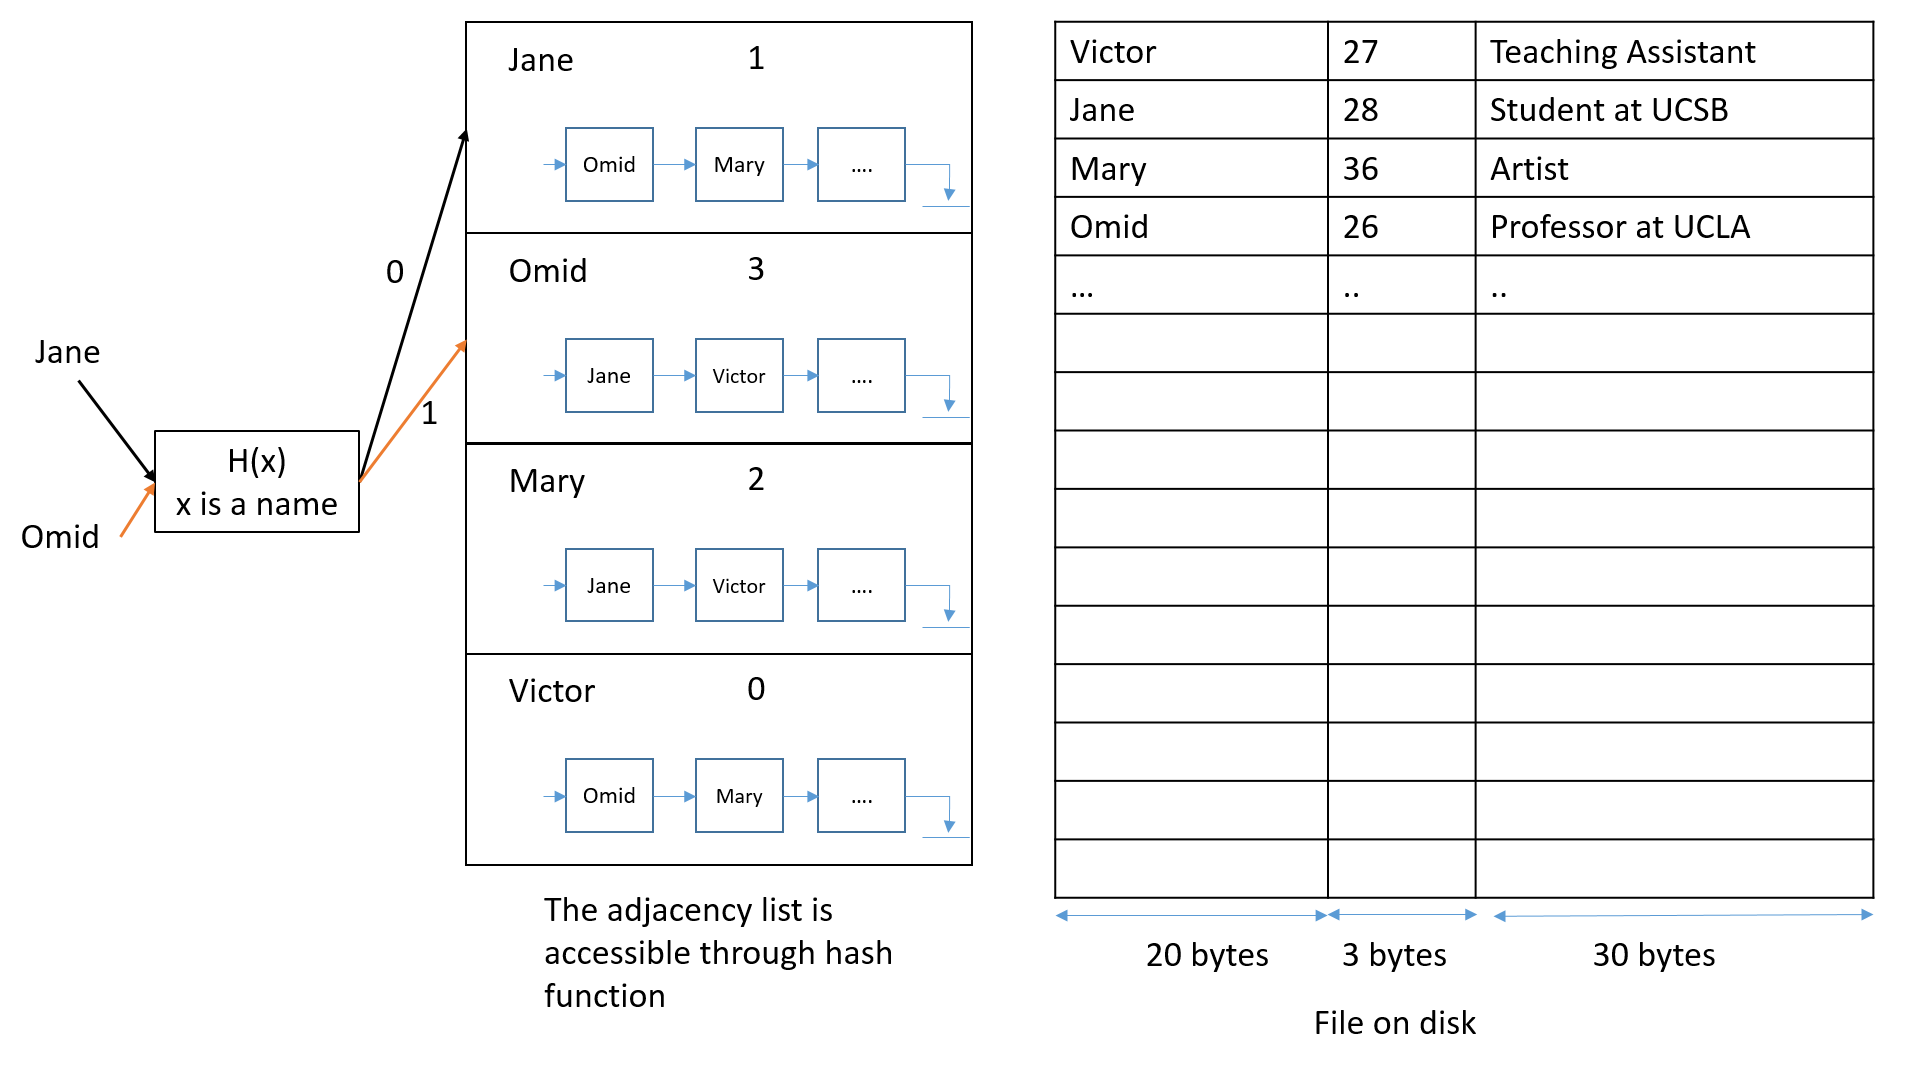
\includegraphics[width=7in,height=3in]{Architecture_updated}
    \caption{Friendship Graph architecture}
    \label{fig:graph}
\end{figure}

\subsection{Profile Data}
The data records are stored in a file on disk. All records have the same size and format. Therefore, you can use the following structure for your file for each user:
\begin{lstlisting}[language=C++,
    directivestyle={\color{black}}
    emph={int,char,double,float,unsigned},
    emphstyle={\color{green}}
    ]
char[20] name;
char[3] age;
char[30] occupation;
\end{lstlisting}

Note that since the size of each record is known, you can simply seek to any record you want in the file on the hard disk. %Property \textit{picturePath} has a system path to a picture (for instance picutres/mike.jpg).
A B-Tree is defined on the {\bf unique} {\em name} attribute, which means that the key for the B-tree is {\em name}. Hence, we should be able to search for one specific name as well as a range of names (for instance Hilda to Omid inclusive). For uniformity, and to ensure that you exhibit interesting splitting cases, your B-tree should be designed with M=5 and L=3. See Figure~2 for an example of such a B-tree.  It has 12 data items, corresponding to 12 people.  The leaves of the tree contain the name of a user and a pointer (index) into the Profile Data file (on disk) for this user's record.

It is highly encouraged to link the leaves to each other to simplify a sorted traverse over all records. This modification of a B-Tree is called a B+Tree and it is extremely useful for range queries. To do this, you can add a pointer to each leaf which points to the next (right) leaf.

For easiness in debugging, the output of {\em PrintAll} function should be similar to the following, each user's information on a separate line.

Mary,21,Developer,Jane,Alex,Ben

Alex,40,School Teacher,Mary,Mike


\begin{figure}[H]
    \centering
    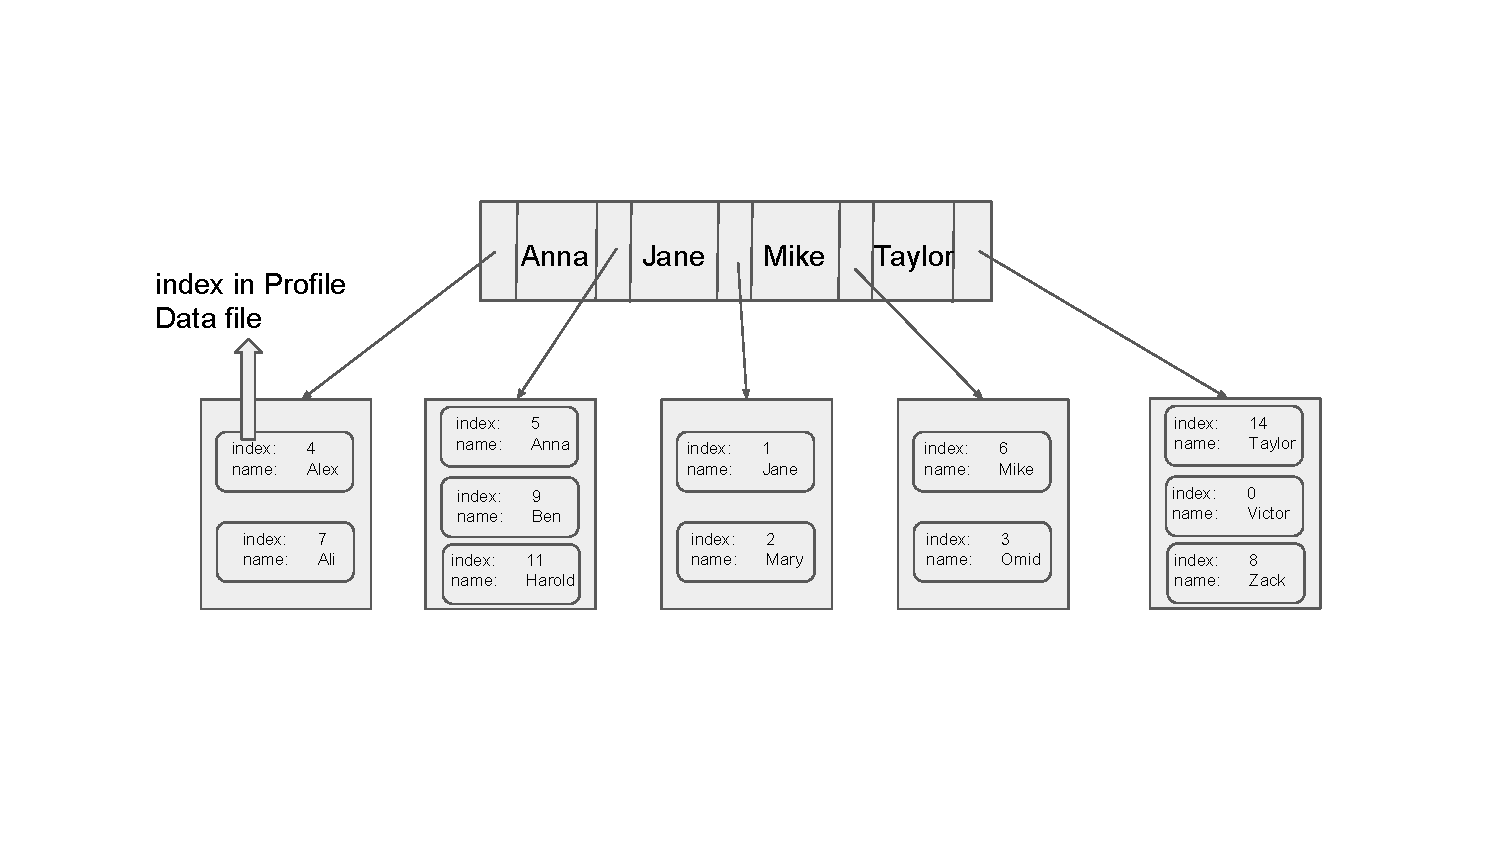
\includegraphics[width=7in,height=3in]{B-Tree_Sample}
    \caption{B-Tree sample structure}
    \label{fig:btree}
\end{figure}


\subsection{Handin}
\begin{itemize}
    \item For this project, you can work in groups of 2 students. Groups should demo their project on the course's final demo date, {\bf Monday March 14}. Hence, there is no need to enforce a single input and output format.
\end{itemize}
\textbf{Minimum Requirements Summary:}
\begin{itemize}
    \item Your program should be able to initialize the adjacency list, the B-tree, and the Profile Data file from an input file that includes a list of users, their attributes, i.e., their name, age, occupation, and a list of their friends' names. The format will be simple, a list (separated by comma) of\\
    $name,age,occupation,friend1,friend2,friend3 \cdots$ each on a single line. Note that name and occupation potentially can have spaces.
    \item You will also use a similar file to initialize your program during the demo.
    \item Insert a new user to the network e.g. Insert Mic 25 "Student at UCSB". 
    \item Add a Friendship relationship between 2 users: AddFriend Mic Jane, \textbf{where Mic and Jane have to be already in the network}.
    \item PrintAll
    \item List Names Age Occupation of friends of some user. ListFriendsInfo Omid, \textbf{where Omid has to be already in the network}
    \item List all users' information with names e.g. Alice $\le$ Name $\le$ Bob, ListInfo \textit{lowerBound} \textit{upperBound}, where lowerBound and upperBound are names that may or may not be in the system. 
    \item There is no defined structure for queries; thus, you can define your own syntax. Your software is supposed to at least handle these queries but you can add more queries and add more data structures to make it faster. Your creativity will be greatly appreciated and highly encouraged.
    \item It is worth saying that we tried not to limit you in this project. This is the final project and you can use your creativity, programming skills and even graphical interface design as much as you want :)
\end{itemize}

\end{document}